\section{Gradient Descent} 

  Note that gradient computation is generally very expensive and not scalable as $n$ gets high. Given a dataset $\mathcal{D} = \{d_i\}_i$ of $D$ points, our posterior is of the form $p(\theta \mid \mathcal{D}) \propto p(\mathcal{D} \mid \theta) \, p(\theta)$ and so 
  \begin{equation}
    \nabla_\theta \log p(\theta \mid \mathcal{D}) = \nabla_\theta \log{p(\theta)} + \nabla_\theta \log{p(\mathcal{D} \mid \theta)} = \nabla_\theta \log{p(\theta)} + \sum_i \nabla_\theta \log{p(d_i \mid \theta)}
  \end{equation}

  We can approximate this gradient by taking a minibatch of $\mathcal{D}$. Let us take a minibatch of $m$ samples $M_m (\mathcal{D})$ without replacement, where $m << D$. Then, our approximation of the gradient of the log likelihood is 

  \begin{equation}
    \nabla_\theta \log{p(\mathcal{D} \mid \theta)} \approx \nabla_\theta \log{p (M_m (\mathcal{D}) \mid \theta)} \coloneqq \frac{D}{m} \sum_{d \in M_m(\mathcal{D})} \nabla_\theta \log{p(d \mid \theta)}
  \end{equation}

  and thus our noisy gradient approximation of the gradient of the log posterior is 

  \begin{equation}
    \nabla_\theta \log{p(\theta \mid \mathcal{D})} \approx \nabla_\theta \log{p(\theta \mid M_m(\mathcal{D}))} \coloneqq \nabla_\theta \log{p(\theta)} + \nabla_\theta \log{p (M_m (\mathcal{D}) \mid \theta)}
  \end{equation}

\subsection{SGD} 

  The classical gradient ascent algorithm simply optimizes a concave function, or if $f$ is multimodal, finds a local maxima. When we use the entire $\mathcal{D}$ to compute the gradient, we call this a \textit{batch gradient descent}, and if the minibatch estimate of the gradient is used, then this is called \textit{stochastic gradient descent}. Ideally, we would want to have a variable step size $h(t)$ so that $h \rightarrow 0$ as $t \rightarrow + \infty$. 

  \begin{algorithm}
    \caption{Stochastic Gradient Ascent}\label{alg:sgd}
    \begin{algorithmic}

    \Require Initial $\boldsymbol{\theta}_0$, Stepsize function $h(t)$, Minibatch size $m$

    \For{$t = 0$ to $T$ until convergence,}
        \State $\hat{g}(\theta_t) \gets \nabla_\theta \log{p(\theta_t \mid M_m(\mathcal{D}))}$
        \State $\theta_{t+1} \gets \theta_t + h(t) \cdot \hat{g}(\theta_t)$
    \EndFor

    \end{algorithmic}
  \end{algorithm}

  SGD with momentum. 

  We have assumed knowledge of gradient descent in the back propagation step in the previous section, but let's revisit this by looking at linear regression. Given our dataset $\mathcal{D} = \{\mathbf{x}^(n), y^{(n)}\}$, we are fitting a linear model of the form 
  \begin{equation}
    f(\mathbf{x}; \mathbf{w}, b) = \mathbf{w}^T \mathbf{x} + b
  \end{equation} 
  The squared loss function is 
  \begin{equation}
    \mathcal{L}(\mathbf{w}, b) = \frac{1}{2} \sum_{n=1}^N \big( y - f(\mathbf{x}; \mathbf{w}, b) \big)^2 = \frac{1}{2} \sum_{n=1}^N \big( y - (\mathbf{w}^T \mathbf{x} + b) \big)^2  
  \end{equation}
  If we want to minimize this function, we can visualize it as a $d$-dimensional surface that we have to traverse. Recall from multivariate calculus that the gradient of an arbitrary function $\mathcal{L}$ points in the steepest direction in which $\mathcal{L}$ increases. Therefore, if we can compute the gradient of $\mathcal{L}$ and step in the \textit{opposite direction}, then we would make the more efficient progress towards minimizing this function (at least locally). The gradient can be solved using chain rule. Let us solve it with respect to $\mathbf{w}$ and $b$ separately first. Beginners might find it simpler to compute the gradient element-wise. 
  \begin{align}
    \frac{\partial}{\partial w_j} \mathcal{L}(\mathbf{w}, b) 
    & = \frac{\partial}{\partial w_j} \bigg(\frac{1}{2} \sum_{n=1}^N \Big( f (\mathbf{x}^{(n)}; \mathbf{w}, b) - y^{(n)} \Big)^2 \bigg) \\
    & = \frac{1}{2} \sum_{n=1}^N \frac{\partial}{\partial w_j} \Big( f(\mathbf{x}^{(n)}; \mathbf{w}, b) - y^{(n)}\Big)^2 \\
    & = \frac{1}{2} \sum_{n=1}^N 2 \Big( f(\mathbf{x}^{(n)}) - y^{(n)}\Big) \cdot \frac{\partial}{\partial w_j} \big( f(\mathbf{x}^{(n)}; \mathbf{w}, b) - y^{(n)} \big) \\
    & = \frac{1}{2} \sum_{n=1}^N 2 \Big( f(\mathbf{x}^{(n)}) - y^{(n)}\Big) \cdot \frac{\partial}{\partial w_j} \big( \mathbf{w}^T \mathbf{x}^{(n)} + b - y^{(n)} \big) \\
    & = \sum_{n=1}^N \big( f(\mathbf{x}^{(n)}; \mathbf{w}, b) - y^{(n)}\big) \cdot x_j^{(n)} \;\;\;\;\;(\text{for } j = 0, 1, \ldots, d)
  \end{align}
  As for getting the derivative w.r.t. $b$, we can redo the computation and get 
  \begin{equation}
    \frac{\partial}{\partial w_j}\mathcal{L}(\mathbf{w}, b) = \sum_{n=1}^N \big( f (\mathbf{x}^{(n)}; \mathbf{w}, b) - y^{(n)}\big) 
  \end{equation}
  and in the vector form, setting $\boldsymbol{\theta} = (\mathbf{w}, b)$, we can set 
  \begin{align}
    \nabla \mathcal{L} (\mathbf{w}) & = \mathbf{X}^T (\hat{\mathbf{y}} - \mathbf{y}) \\
    \nabla \mathcal{L} (b) & = (\hat{\mathbf{y}} - \mathbf{y}) \cdot \mathbf{1}
  \end{align}
  where $\hat{\mathbf{y}}_n = f(\mathbf{x}^{(n)}; \mathbf{w}, b)$ are the predictions under our current linear model and $\mathbf{X} \in \mathbb{R}^{n \times d}$ is our design matrix. This can easily be done on a computer using a package like \texttt{numpy}. Remember that GD is really just an algorithm that updates $\boldsymbol{\theta}$ repeatedly until convergence, but there are a few problems.
  \begin{enumerate}
    \item The algorithm can be susceptible to local minima. A few countermeasures include shuffling the training set or randomly choosing initial points $\theta$
    \item The algorithm may not converge if $\alpha$ (the step size) is too high, since it may overshoot. This can be solved by reducing the $\alpha$ with each step, using \textit{schedulers}. 
    \item The entire training set may be too big, and it may therefore be computationally expensive to update $\boldsymbol{\theta}$ as a whole, especially if $d >> 1$. This can be solved using stochastic gradient descent.
  \end{enumerate}

  Rather than updating the vector $\boldsymbol{\theta}$ in batches, we can apply \textbf{stochastic gradient descent} that works incrementally by updating $\boldsymbol{\theta}$ with each term in the summation. That is, rather than updating as a batch by performing the entire matrix computation by multiplying over $N$ dimensions,
  \begin{equation}
    \nabla \mathcal{L} (\mathbf{w}) = \underbrace{\mathbf{X}^T}_{D \times N} \underbrace{(\hat{\mathbf{y}} - \mathbf{y})}_{N \times 1}
  \end{equation}
  we can reduce this load by choosing a smaller subset $\mathcal{M} \subset \mathcal{D}$ of $M < N$ elements, which gives 
  \begin{equation}
    \nabla \mathcal{L}_{\mathcal{M}} (\mathbf{w}) = \underbrace{\mathbf{X}_{\mathcal{M}}^T}_{D \times M} \underbrace{(\hat{\mathbf{y}_{\mathcal{M}}} - \mathbf{y}}_{\mathcal{M}})_{M \times 1}
  \end{equation}
  The reason we can do this is because of the following fact.  
  
  \begin{theorem}[Unbiasedness of SGD]
    $\nabla \mathcal{L}_{\mathcal{M}} (\mathbf{w})$ is an \textit{unbiased estimator} of the true gradient. That is, setting $\mathcal{M}$ as a random variable of samples over $\mathcal{D}$, we have 
    \begin{equation}
      \mathbb{E}_{\mathcal{M}} [\nabla \mathcal{L}_{\mathcal{M}} (\mathbf{w})] = \nabla \mathcal{L} (\mathbf{w})
    \end{equation}
  \end{theorem}
  \begin{proof}
    We use linearity of expectation for all $\mathcal{M} \subset \mathcal{D}$ of size $M$. 
  \end{proof}

  Even though these estimators are noisy, we get to do much more iterations and therefore have a faster net rate of convergence. By using repeated chain rule, or a fancier term is automatic differentiation, as shown before, SGD can be used to optimize neural networks. 

  Extending beyond SGD, there are other optimizers we can use. Essentially, we are doing a highly nonconvex optimization, which doesn't have a straightforward answer, so the best we can do is play around with some properties. 0th order approximations are hopeless since the dimensions are too high, and second order approximations are hopeless either since computing the Hessian is too expensive for one run. Therefore, we must resort to some first order methods, which utilize the gradient. Some other properties to consider are: 
  \begin{enumerate} 
    \item Learning rate 
    \item Momentum 
    \item Batch Size
  \end{enumerate}

\subsection{RMSProp} 

\subsection{Adam} 

\subsection{Adagrad}

\subsection{Nesterov Momentum}

\subsection{Sparsity-Inducing SGD} 

  We can do SGD with clipping. 

\subsection{Block Coordinate Descent} 

\subsection{Proximal Gradient Descent}

  \subsubsection{Subdifferentials}

    \begin{definition}[Convex Function]
      A function $f: U \subset \mathbb{R}^n \rightarrow \mathbb{R}$ defined on a convex set $U$ is convex if and only if for any $\mathbf{x}, \mathbf{y} \in U$
      \begin{equation}
        f \big(\lambda \mathbf{x} + (1 - \lambda) \mathbf{y} \big) \leq \lambda f(\mathbf{x}) + (1 - \lambda) f(\mathbf{y})
      \end{equation}
      Now if $f$ is differentiable, then convexity is equivalent to 
      \begin{equation}
        f(x) \geq f(y) + \nabla f(y)^T \cdot (x - y)
      \end{equation}
      for all $x, y \in U$. That is, its local linear approximation always underestimates $f$. 
    \end{definition}

    It is well known that the mean square error of a linear map is convex. However, when we impose the L1 penalty, the loss function is now not differentiable at $\mathbf{0}$. Therefore, we must introduce the notion of a subgradient. 

    \begin{definition}[Subgradient]
      The subgradient of a convex function $f: U \subset \mathbb{R}^n \rightarrow \mathbb{R}$ is any linear map $\mathbf{A} (x): \mathbb{R}^n \rightarrow \mathbb{R}$ such that 
      \begin{equation}
        f(\mathbf{y}) \geq f(\mathbf{x}) + \mathbf{A}(\mathbf{x}) (\mathbf{y} - \mathbf{x})
      \end{equation}
      for any $\mathbf{y} \in U$. The set of all subgradients at $\mathbf{x}$ is called the \textbf{subdifferential} defined 
      \begin{equation}
        \partial f (\mathbf{x}) = \{ \mathbf{A} \in \mathbb{R}^n \mid \mathbf{A} \text{ is a subgradient of } f \text{ at } \mathbf{x} \}
      \end{equation}
    \end{definition}

    The subgradient also acts as a linear approximation of $f$, but now at nondifferentiable points of convex functions, we have a set of linear approximations. It is clear that the subgradient at a differentiable point is uniquely the gradient ($\partial f(\mathbf{x}) = \{ \nabla f(\mathbf{x})$), but for places like the absolute value, we can have infinite linear approximations. 
    \begin{center}
      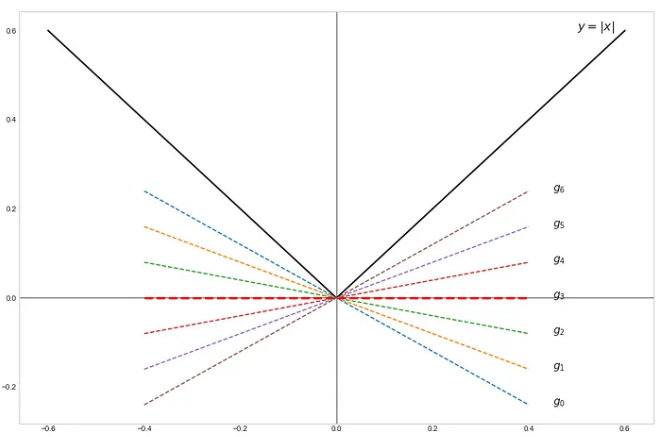
\includegraphics[scale=0.4]{img/subgradient_of_abs.png}
    \end{center}
    Given the subdifferential, thus the optimality condition for any convex $\mathbf{f}$ (differentiable or not) is
    \begin{equation}
      f(\mathbf{x}^\ast) = \min_{\mathbf{x}} f(\mathbf{x}) \iff \mathbf{0} \in \partial f(\mathbf{x}^\ast)
    \end{equation}
    known as the subgradient optimality condition, which clearly implies 
    \begin{equation}
      f(\mathbf{y}) \geq f(\mathbf{x}^\ast) + \mathbf{0}^T (\mathbf{y} - \mathbf{x}^\ast) = f(\mathbf{x}^\ast)
    \end{equation}

    \begin{example}
      The subdifferential of the absolute value function $f(x) = |x|$ at any given $x$ is 
      \begin{equation}
        \partial f(x) = \begin{cases} 1 & \text{ if } x > 0 \\ [-1, 1] & \text{ if } x = 0 \\ -1 & \text{ if } x < 0 \end{cases}
      \end{equation}
    \end{example}

  \subsubsection{Proximal Operators and Soft Thresholding}

    \begin{definition}[Proximal Operator]
      Given a lower semicontinuous convex function $f$ mapping from Hilbert space $X$ to $[-\infty, +\infty]$, its \textbf{proximal operator} associated with a point $u$ is defined 
      \begin{equation}
        \prox_{f, \tau} (u) = \argmin_{x} \bigg( f(x) + \frac{1}{2\tau} ||x - u||^2 \bigg)
      \end{equation}
      where $\tau > 0$ is a parameter that scales the quadratic term. This is basically the point that minimizes the sum of $f(x)$ and the square of the Euclidean distance between $x$ and $u$, scaled by $1/2\tau$. 
    \end{definition}

    Now given the loss function $L (\boldsymbol{\theta}) = L_{\mathrm{obj}} (\boldsymbol{\theta}) + L_{\mathrm{reg}} (\boldsymbol{\theta})$, we want to compute the proximal operator on the regularization loss and update that with the gradient of the smooth objective loss. 
    \begin{equation}
      \boldsymbol{\theta}^{(k+1)} = \prox_{L_{\mathrm{reg}}, \tau} \big[ \boldsymbol{\theta}^{(k)} - \tau \nabla L_{\mathrm{obj}} (\boldsymbol{\theta}^{(k)}) \big]
    \end{equation}
    Let's compute the proximal operator of the L1 loss $h(\boldsymbol{\theta}) = \lambda ||\boldsymbol{\theta}||_1$. We can parameterize this loss by the $\lambda$, so we will use the notation $\prox_{\lambda, \tau}$ rather than $\prox_{h, \tau}$. 
    \begin{align*}
      \prox_{\lambda, \tau} (\mathbf{u}) & = \argmin_{\boldsymbol{\theta}} \bigg( \lambda ||\boldsymbol{\theta}||_1 + \frac{1}{2\tau} ||\boldsymbol{\theta} - \mathbf{u}||_2^2 \bigg) \\
      & = \argmin_{\boldsymbol{\theta}} \bigg( \sum_{i=1}^n \lambda |\theta_i| + \frac{1}{2\tau} (\theta_i - u_i)^2 \bigg) 
    \end{align*}
    These are separable functions that can be decoupled and optimized component-wise. So, we really just want to find 
    \begin{equation}
      \theta_i^\ast = \argmin_{\theta_i} \bigg( \lambda |\theta_i| + \frac{1}{2\tau} (\theta_i - u_i)^2 \bigg)
    \end{equation}
    The sum of convex functions is convex, and so we should differentiate it and find where the gradient is $0$ to optimize it. 
    \begin{enumerate}
      \item When $\theta_i > 0$, then we minimize $\lambda \theta_i + \frac{1}{2\tau} (\theta_i - u_i)^2$, so taking the gradient and setting to $0$ gives 
      \begin{equation}
        \theta_i = u_i - \lambda \tau
      \end{equation}
      subject to the constraint that $\theta_i > 0$, or equivalently, that $u_i > \lambda \tau$. 

      \item When $\theta_i < 0$, then we minimize $-\lambda \theta_i + \frac{1}{2\tau} ( \theta_i - u_i)^2$, so taking the gradient and setting to $0$ gives 
      \begin{equation}
        \theta_i = u_i + \lambda \tau
      \end{equation}
      subject to the constraint that $\theta_i < 0$, or equivalently, that $u_i < -\lambda \tau$. 

      \item When $\theta_i = 0$, then we minimize $\lambda |\theta_i| + \frac{1}{2\tau} (\theta_i - u_i)^2$, which doesn't have derivative at $\theta_i = 0$. So, we can compute the subdifferential of it to get 
      \[0 \in \partial \bigg( \lambda |\theta_i| + \frac{1}{2\tau} (\theta_i - u_i)^2 \bigg) = \lambda \partial (|\theta_i|) + \frac{1}{\tau} (\theta_i - u_i)\]
      Now at $\theta_i = 0$, the subdifferential can be any value in $[-1, 1]$, and the above reduces to 
      \begin{equation}
        0 \in \lambda [-1, 1] - \frac{1}{\tau} u_i
      \end{equation}
      this is equivalent to saying that $u_i/\tau$ is contained in the interval $[-\lambda, \lambda]$, meaning that $u_i \in [-\lambda \tau, \lambda \tau]$. 
    \end{enumerate}

    Ultimately we get that 
    \begin{equation}
      \prox_{\lambda, \tau} (u) = \begin{cases} u - \lambda \tau & \text{ if } u > \lambda \tau \\ 0 & \text{ if } |u| \leq \lambda \tau \\ u + \lambda \tau & \text{ if } u < - \lambda \tau \end{cases}
    \end{equation}
    which can be simplified to 
    \begin{equation}
      \prox_{\lambda, \tau} (u) = \mathrm{sign}(u) \max\{ |u| - \lambda \tau, 0)
    \end{equation}

